\section{Introduction}
\label{sec:intro}

In order to meet the increasing needs for food and materials, researchers aim to produce sustainable plants with high yield and high resource-use efficiency by testing approaches ranging from molecular biology to field management~\cite{walter2015plant1}. In this process high-throughput plant phenotyping is the major bottleneck~\cite{cobb2013next}. New automated methods to non-invasively measure plant phenotypes including growth, plant structure, leaf layout and orientations, photosynthesis and productivity, are highly expected~\cite{leister1999large,muller2015leaf,walter2015plant1}. 


\begin{figure}
\begin{center}
\begin{tabular}{ c c }
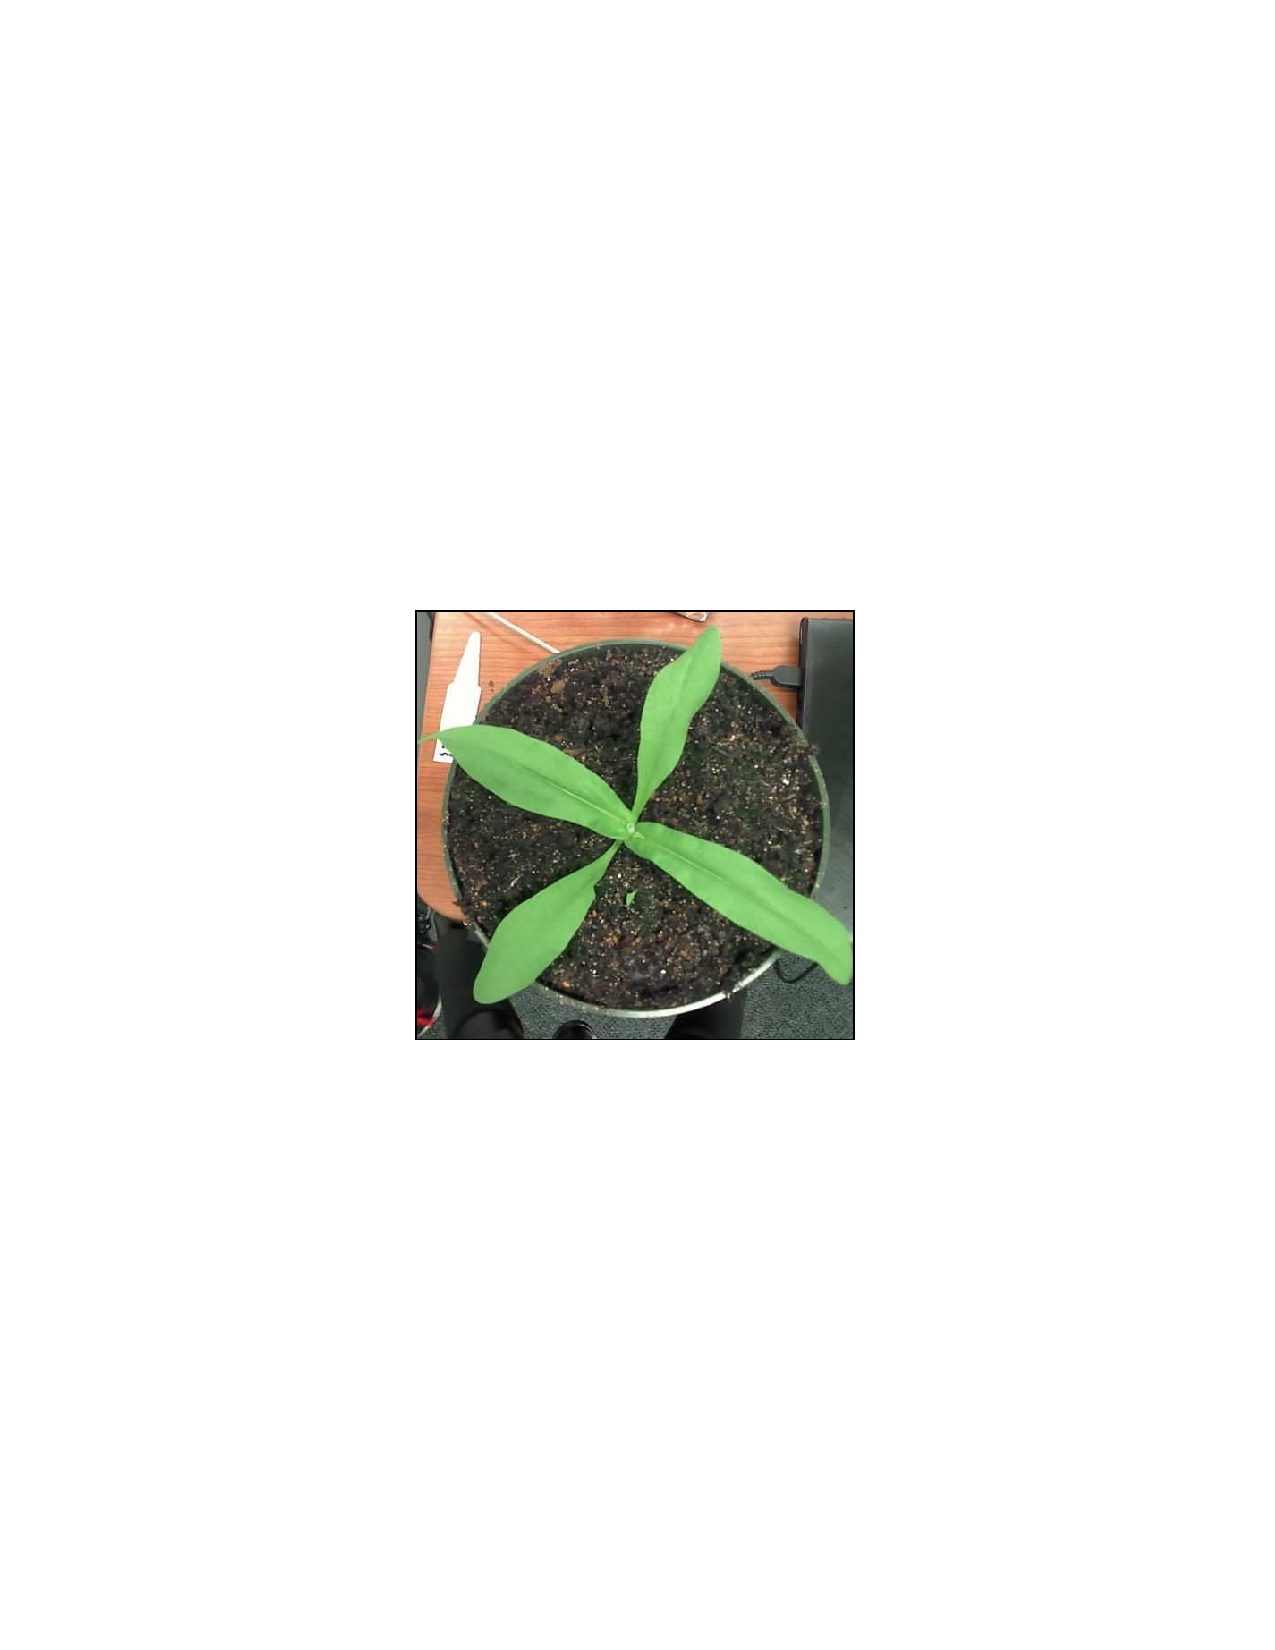
\includegraphics[trim=200 280 200 280,clip,width=0.4\linewidth]{Figures/plant1-rgb} &
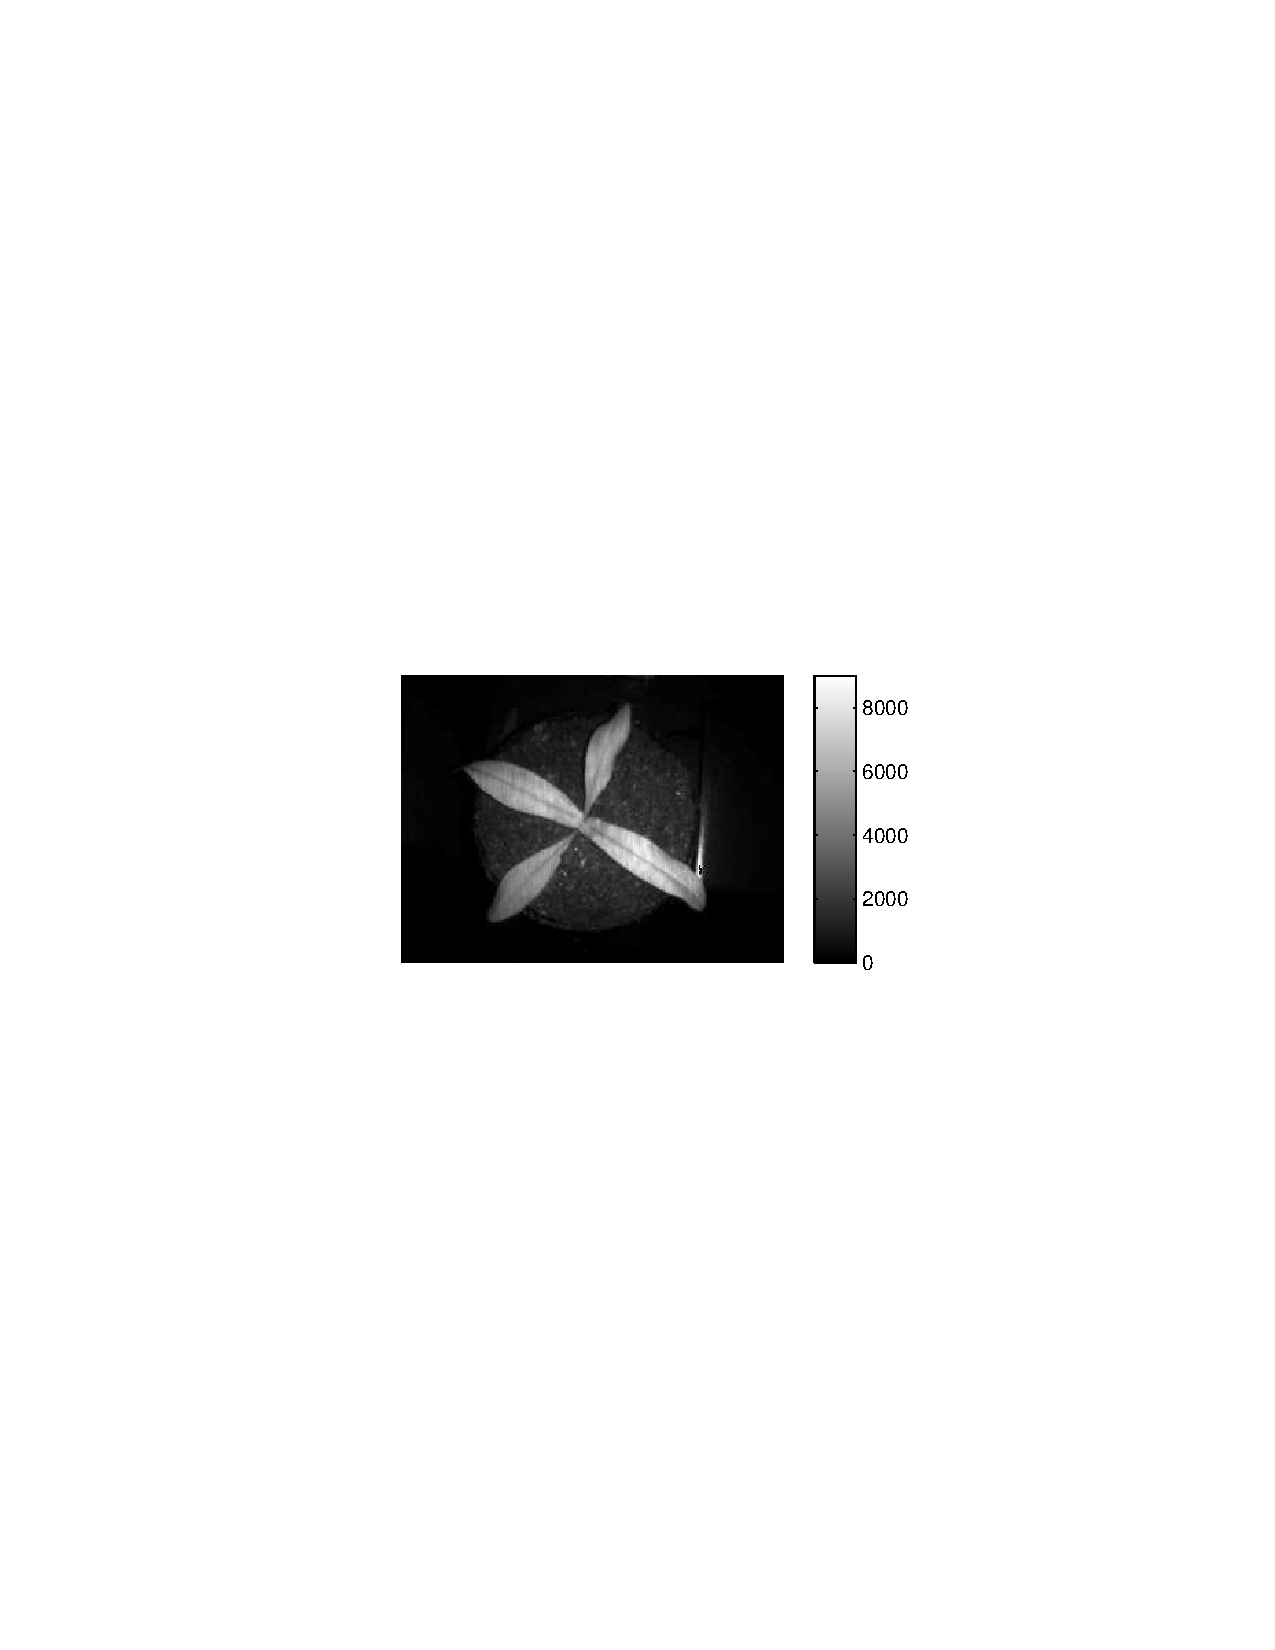
\includegraphics[trim=220 270 160 280,clip,width=0.4\linewidth]{Figures/plant1-ir} \\
($a$) & ($b$) \\
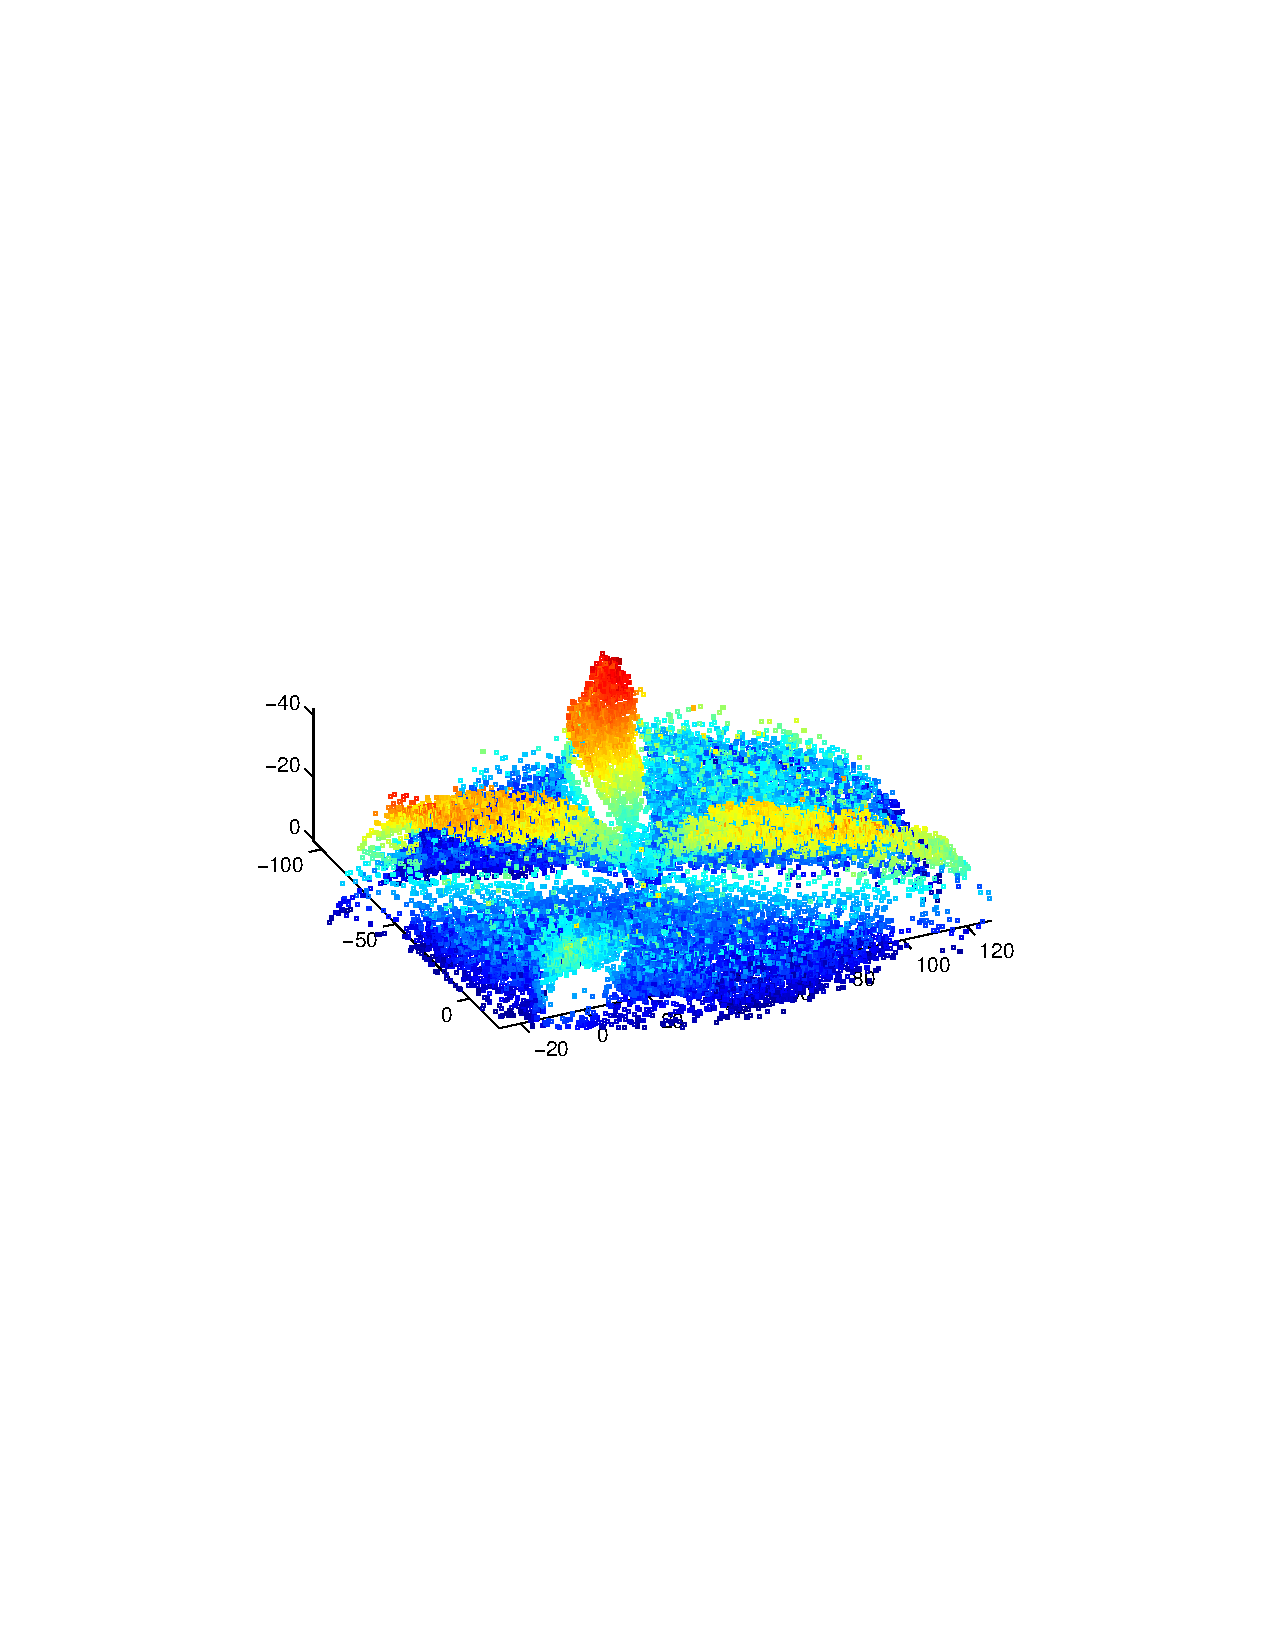
\includegraphics[trim=180 270 180 280,clip,width=0.4\linewidth]{Figures/plant1-noise} &
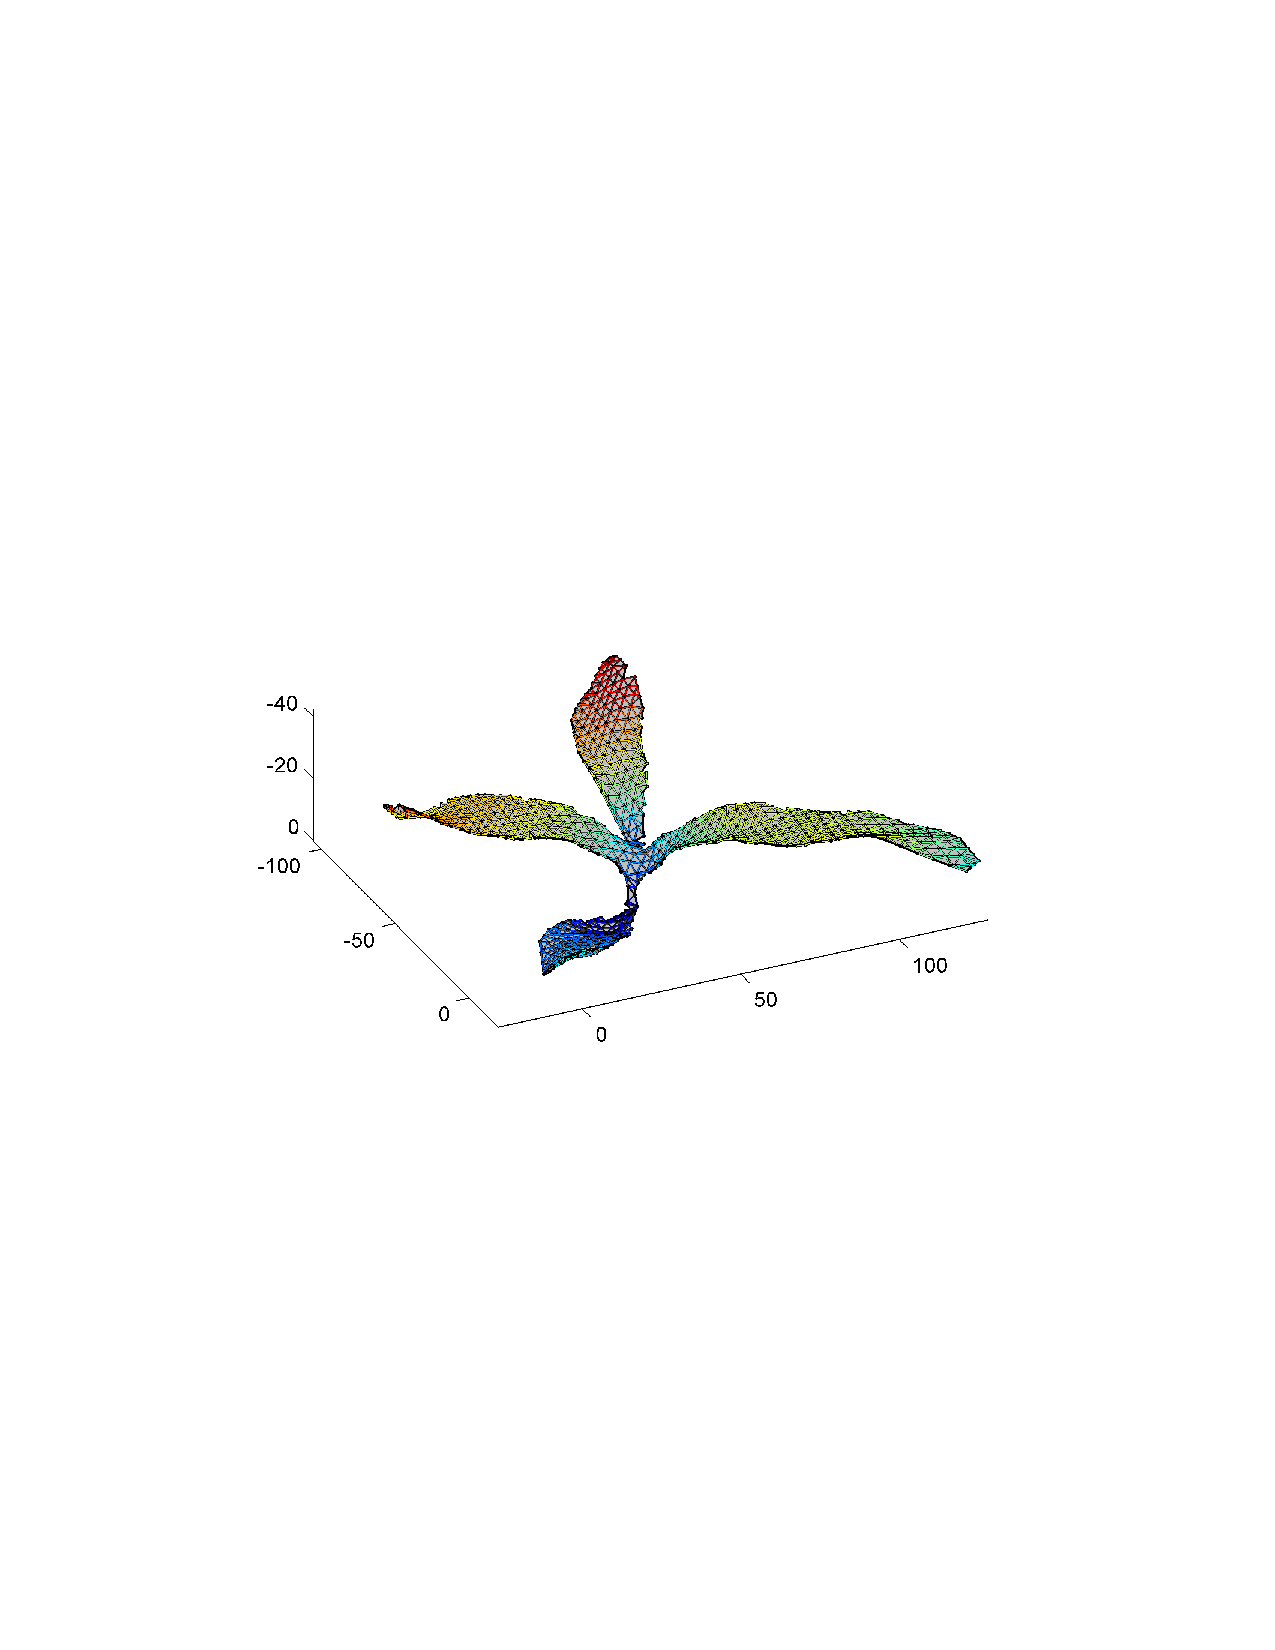
\includegraphics[trim=180 270 180 280,clip,width=0.4\linewidth]{Figures/plant1-mesh} \\
($c$) & ($d$) \\
\end{tabular}
\end{center}
\caption{Illustration of sensor data.  ($a$) Portion of color image. ($b$) IR reflectance image with reflectance values. ($c$) Portion of a single depth image surrounding plant averaged over 60 frames to reduce noise, and projected into $3$D showing significant remaining depth noise. ($d$)  The mesh resulting from the algorithm in this paper using data from the color, depth and IR reflectance images.  Units of $3$D plots are mm.  }
\label{fig:plantnoise}
\end{figure}


An important step in estimating all of the plant phenotypic properties is to obtain $3$D shape and pose for all the plant leaves~\cite{muller2015leaf}, which has to be measured in a limited growth space with minimum disturbance, making it impractical to use scanning lasers for shape modeling. As an alternative, we propose to mount close-range time-of-flight RGB-D sensors in the growth chambers, acquire color, IR-reflectance and range data, and estimate leaf shape through building leaf $3$D mesh models (see Fig.~\ref{fig:plantnoise}). Mesh fitting to $3$D point clouds and depth maps enables visualization and leaf shape analysis by providing a surface topology and geometry to a point cloud~\cite{Sienz2000,Yeh2011}.  A mesh can efficiently compress dense scanned data and mesh fitting methods have been developed that adhere to the underlying shape and preserve geometric features such as creases~\cite{hoppe:1994,Kobbelt:1998}. 
%
However, while time-of-flight RGB-D sensors are small, inexpensive and provide dense $3$D surface sampling of objects, they pose a challenge to surface modeling of small objects due to large depth noise. Specifically, in our leaf $3$D mesh modeling application, the pixel-depth noise has a standard deviation on the order of the surface feature sizes (see Fig.~\ref{fig:sigmainterframe}). In this paper, we present a new solution to automatically build precise $3$D mesh models of plant leaves using time-of-flight RGB-D sensors. We achieve this through formulating an optimization that minimizes depth noise and adds a curvature-based regularization.  

There have been differing goals in previous work on automated $3$D leaf modeling.   One goal has been to generate realistic foliage for graphics~\cite{Bradley:2013}.  Here known leaf shapes are fit to $3$D structure from motion data producing realistic-looking foliage, but not necessarily a close approximation to the actual plant leaf shapes and poses.  In~\cite{Quan:2006} an interactive system enables semi-automatic estimation of complex arrangements of leaves.  The leaf shapes are all very similar and are fit by warping a template.  In~\cite{Alenya2011,Alenya2013} plant leaves are automatically segmented and fit using color and time-of-flight data enabling robotic arm inspection.  This work is most similar to ours and they use a similar sensor, but the goals are quite different.  They automatically segment and estimate poses of densely spaced leaves using simple geometric models (planes and parabolas) to fit the 3D data resulting in leaf poses and rough shape approximations.  Our goal, on the other hand, is not segmenting overlapping leaves, but rather to estimate complex $3$D leaf surfaces as precisely as possible from the noisy data.  For this our flexible mesh model fitting approach gives much more accurate results.



%Another goal for mesh fitting is to incrementally build full $3$D models of objects.  Zippered polygons~\cite{Turk1994} builds mesh models from range images and combines them discarding noisy points at the boundaries.  The method developed by Curless and Levoy~\cite{Curless:1996} populates a weighted voxel occupancy grid from the depth data and recovers the surface by triangulating an isosurface.  By raycasting this surface, new camera poses can be aligned and their depths maps contribute to and improve the voxel model.  Advantages of this method include that surface topology is automatically determined, additional data can be readily incorporated, holes can be filled when more data are collected and it incorporates directional uncertainty of range data into the models.  Recent approaches for environment modeling from RGB-D cameras such as Kinect Fusion~\cite{Izadi:2011,Newcombe:2011} build on this voxel modeling and accumulation.  For our application the sensor is fixed and there is no option for merging views from different perspectives.  Artifacts caused by discretization into voxels are significant particularly with high input noise, and the method is limited in incorporating surface smoothness priors. .......MOVE TO RELATED WORK

We propose a new mesh generation algorithm that has the following advantages:
\begin{itemize}
\item It resolves complex $3$D leaf shapes despite large noise in the range images by leveraging multiple sensor modalities.  
\item Boundary edge features in the high resolution color image are used to help select and constrain vertices and mesh edges.  
\item The errors in depth are modeled along camera rays and minimized during fitting to facets.  
\item A regularization term modeling curvature is incorporated and a linear approximation enables a fast, least-squares shape fit.
\end{itemize}



